% ch04 —— 第 4 章 並河良典「カラビ--ヤウ多様体と代数幾何」
% 本章原书节号用阿拉伯数字（1, 2, …），而 preamble 默认 \thesection 为罗马数字。
% 章内局部改写为阿拉伯数字，章末再恢复（Lead 已裁定；见 reports/ch04.md）。
\renewcommand{\thesection}{\arabic{section}}
\chapter{Calabi--Yau 流形与代数几何}
\chapterauthor{並河良典}{[京都大学大学院理学研究科]}

% ===== PDF p.054 (原书 p.46) =====
\section{代数簇的分类与 Calabi--Yau 流形}

这里，我们要说明 Calabi--Yau 流形在整个代数簇的世界里处在什么位置。以下，除非特别声明，所谓代数簇，都限定为作为闭集嵌入复射影空间、并且没有奇点的对象。射影空间上有一个叫作 Fubini--Study 度量的 Kähler 度量，把它限制上去，代数簇就成为 Kähler 流形。Calabi--Yau 流形 $X$，指的是典范丛 $K_X$ 平凡的代数簇。设 $X$ 是 Calabi--Yau 流形、$\omega$ 是 $X$ 上的 Kähler 度量，那么就存在唯一一个 Ricci 平坦的 Kähler 度量 $\omega_0$，满足 $[\omega_0] = [\omega] \in H^2(X,\R)$。这是 Calabi（E. Calabi）提出猜想、Yau（S. T. Yau）给出证明的大定理。Calabi--Yau 流形这个名字就来自这个结果。

代数几何的一个目标，是弄清代数簇有哪些种类。以下，我们来看 Calabi--Yau 流形在代数簇的分类理论中是如何出现的。1 维代数簇 $C$ 叫作代数曲线，按亏格 $g(C)$ 大致分成 3 类：

\[
\begin{array}{ll}
g(C) = 0 & \Longrightarrow\ C \cong \PP^1,\\
g(C) = 1 & \Longrightarrow\ C : \text{椭圆曲线},\\
g(C) > 1 & \Longrightarrow\ C : \text{一般型曲线}.
\end{array}
\]

$g(C)=0$ 时，$C$ 的曲率是正的；$g(C)>1$ 时，$C$ 的曲率是负的。而 $g(C)=1$ 时，$C$ 具有平坦的 Kähler 度量，曲率为 0。因此，1 维的 Calabi--Yau 流形只能是椭圆曲线。要处理 2 维以上的代数簇，一个叫作 Kodaira 维数的不变量很有用（飯高茂、Moishezon）。以下就这个概念
% ===== PDF p.055 (原书 p.47) =====
作简单说明。把代数簇 $X$ 的余切丛记作 $\Omega^1_X$。这时，$\Omega^1_X$ 的秩等于 $X$ 的维数 $d$。$X$ 的典范丛 $K_X$，就是把 $\Omega^1_X$ 外积 $d$ 次得到的线丛 $\wedge^d\Omega^1_X$。对自然数 $n>0$，把 $(K_X)^{\otimes n}$ 的整体截面全体构成的 $\C$ 向量空间记作 \(\Gamma(X,(K_X)^{\otimes n})\)。设 \(\Gamma(X,(K_X)^{\otimes n})\) 的一组基为 $s_0,\dots,s_m$，那么就得到从 $X$ 到 $m$ 维射影空间 $\PP^m$ 的有理映射

\[
  \phi_n : X \dashrightarrow \PP^m ,
\]

它由

\[
  \phi_n(p) := (s_0(p) : s_1(p) : \cdots : s_m(p)) \in \PP^m
\]

给出。当然，如果 \(\Gamma(X,(K_X)^{\otimes n}) = 0\)，$\phi_n$ 就没有定义。另外，$\phi_n$ 会随基 $\{s_0,\dots,s_m\}$ 的选取而改变；但只要用 $\mathrm{PGL}(m+1)$ 中适当的元素去变换 $\PP^m$，就可以把改变后的映射看成同一个有理映射。于是，我们如下定义 $X$ 的 Kodaira 维数 $\kappa(X)$。首先，如果对任何 $n>0$ 都有 \(\Gamma(X,(K_X)^{\otimes n}) = 0\)，就定义

\[
  \kappa(X) = -\infty .
\]

另一方面，如果至少存在一个 $n$ 使 \(\Gamma(X,(K_X)^{\otimes n}) \neq 0\)，就定义

\[
  \kappa(X) = \max_{n>0}\{\dim \phi_n(X)\} .
\]

这时 $\kappa(X)$ 是 $X$ 的双有理不变量。也就是说，把 $X$ 换成双有理等价的另一个 $X'$，Kodaira 维数不变。

下面说明极小模型这个概念。假设代数簇 $X$ 上给定了线丛 $L$ 和曲线 $C$。取 $C$ 的奇点消解 $h : \tilde{C} \to C \subset X$，把 $L$ 与 $C$ 的相交数 $(L.C)$ 定义为

\[
  (L.C) = \int_C h^* c_1(L) .
\]

如果对所有的曲线 $C \subset X$ 都有 $(L.C) \ge 0$，这样的线丛 $L$ 就叫作 nef（数值正）的。典范丛 $K_X$ 是 nef 的代数簇 $X$，叫作极小的。对给定的代数簇 $Y$，如果存在与 $Y$ 双有理等价的极小代数簇 $X$，就把 $X$ 叫作 $Y$ 的极小模型。在 2 维以上代数簇的分类里，这两个概念（Kodaira 维数、极小模型）起重要作用。先来看代数曲面的情形。代数曲面 $S$ 上的曲线 $C$，若满足 $(K_S.C) = -1$、$C \cong \PP^1$，就
% ===== PDF p.056 (原书 p.48) =====
称为 $(-1)$-曲线。在代数曲面的一个点上作爆破，得到的例外曲线是一条有理曲线，它就是 $(-1)$-曲线。反过来，把一条 $(-1)$-曲线 $C$ 收缩成一点，就能从 $S$ 得到一个新的代数曲面 $S_1$。这个操作叫作收缩（blow-down）。这样，从给定的 $S$ 出发，依次收缩 $(-1)$-曲线，就不断得到新的代数曲面：

\[
  S \longrightarrow S_1 \longrightarrow S_2 \longrightarrow \cdots .
\]

每作一次收缩，代数曲面的第二 Betti 数正好减少 1，所以这个操作在有限步后停止。当 Kodaira 维数 $\kappa(S) \ge 0$ 时，这样最终得到的代数曲面 $\bar{S}$ 就是 $S$ 的极小模型。而当 $\kappa(S) = -\infty$ 时，$\bar{S}$ 同构于 $\PP^2$，或者同构于叫作直纹曲面（ruled surface）的曲面。

这里，我们再仔细看看 $\kappa(S)=0$ 的情形。由定义，存在 $n$ 使 $\dim\Gamma(\bar{S},(K_{\bar{S}})^{\otimes n}) = 1$。把这样的 $n$ 中最小的记作 $n_0$。再设 $q(\bar{S}) := \dim H^1(\bar{S},\cO_{\bar{S}})$。这时，Kodaira 维数为 0 的极小代数曲面分类如下：

\[
\begin{array}{ll}
n_0 = 1,\ q = 0 & \Longrightarrow\ \bar{S} : \text{代数的}\ K3\text{ 曲面},\\
n_0 = 1,\ q = 2 & \Longrightarrow\ \bar{S} : \text{阿贝尔曲面},\\
n_0 > 1,\ q = 0 & \Longrightarrow\ \bar{S} : \text{Enriques 曲面},\\
n_0 > 1,\ q = 1 & \Longrightarrow\ \bar{S} : \text{超椭圆曲面}.
\end{array}
\]

其中前两类，典范丛 $K_{\bar{S}}$ 平凡，是 Calabi--Yau 流形。另一方面，后两类只要取适当的平展覆盖，也分别成为代数的 $K3$ 曲面、阿贝尔曲面。所以，Kodaira 维数为 0 的代数曲面的研究，某种意义上就归结为代数的 $K3$ 曲面与阿贝尔曲面这两种 Calabi--Yau 流形的研究。

下面终于要考虑正题——3 维的情形了。遗憾的是，2 维时的剧本不能原样照搬。事实上，人们发现了 Kodaira 维数 $\ge 0$ 的 3 维代数簇，在（非奇异）代数簇的范畴里并不具有极小模型。在这样的困难中，飯高、上野健爾等人开始了高维代数簇的攻坚。正是在这样的土壤上，森理论诞生了。在高维情形，极小模型的候选者不在非奇异代数簇之中，而在带有某种较弱奇点的代数簇之中。这里说的某种较弱奇点，指的是所谓 $Q$-分解的终端奇点（$Q$-factorial terminal singularity）——
% ===== PDF p.057 (原书 p.49) =====
这样的对象。于是，我们如下重新定义极小代数簇。

\begin{center}
（带奇点的）代数簇 $X$ 称为\textbf{极小}，是指 $X$ 只具有 $Q$-分解的终端奇点，并且典范丛 $K_X$\footnote{由于存在奇点，严格说来 $K_X$ 不是线丛，而是叫作 $Q$-线丛的对象。} 是 nef 的。
\end{center}

接着，把考虑的代数簇从非奇异的对象扩大到带 $Q$-分解的终端奇点的对象。要造极小模型，就像代数曲面时收缩 $(-1)$-曲线那样，必须收缩那些妨碍典范丛成为 nef 的坏子簇。当给定流形的 Kodaira 维数为 $-\infty$ 时，这样的子簇有可能覆盖整个流形；但 Kodaira 维数 $\ge 0$ 时不会发生这种情况。特别在 3 维情形，这样的子簇要么是曲面，要么是曲线。收缩曲面时，得到的流形仍然带有 $Q$-分解的终端奇点，所以继续这个操作即可。但是，收缩曲线时，得到的流形带有比终端奇点更坏的奇点。因此，要把操作继续下去，就不能只是收缩曲线，而需要“把该曲线换成别的曲线”这样的修改操作。这个修改操作叫作翻转（flip）。首先要证明翻转的存在，这是第一个课题。再者，收缩曲面的操作会使第二 Betti 数逐个减少，而翻转不改变第二 Betti 数。因此，没有任何地方保证翻转操作会在有限步内结束。保证这一点是第二个课题。这样一套纲领叫作极小模型纲领。极小模型纲领在 1980 年代初由森重文、Reid、川又雄二郎、Shokurov、Kollár 等人研究，结果证明了：在 3 维情形，翻转总是存在，而且这个操作不会无限次持续下去。因此，对 Kodaira 维数 $\ge 0$ 的 3 维代数簇，极小模型必定存在。而且，极小模型的典范丛不只是 nef，还具有下面的性质。

% [Tutor Note: 丰富性定理断言，3 维极小模型 $X$ 的典范除子 $K_X$ 是半丰沛的，即某个倍数 $|(K_X)^{\otimes n}|$ 无基点，从而 $\phi_n$ 是正则映射而不是仅仅有定义的映射。]

\fkstmt{丰富性定理}{（川又，宮岡洋一）}对 3 维极小模型 $X$，
% ===== PDF p.058 (原书 p.50) =====
适当的 $n>0$ 时，$|(K_X)^{\otimes n}|$ 由整体截面生成。换句话说，有理映射

\[
  \phi_n : X \dashrightarrow \PP^n
\]

成为正则映射。

考虑 Kodaira 维数为 0 的 3 维极小模型 $X$。对 $X$，像代数曲面时一样定义 $n_0$ 和 $q$。复习一下，$q$ 叫作非正则数（irregularity），由 $q(X) = \dim H^1(X,\cO_X)$ 定义。首先，把“Kodaira 维数为 0”与丰富性定理合起来，就知道 $(K_X)^{\otimes n_0}$ 是平凡的。如果 $n_0 > 1$，就可以取一个次数为 $n_0$ 的有限覆盖

\[
  \pi : Y \longrightarrow X,
\]

使得 $K_Y$ 平凡。这样的有限覆盖叫作指数 1 覆盖（index 1 cover）。$Y$ 是带奇点的 Calabi--Yau 流形。也就是说，要研究 $n_0 > 1$ 的极小模型，只需研究 $n_0 = 1$ 的极小模型和指数 1 覆盖。

接下来设 $n_0 = 1$。如果 $q > 0$，$X$ 的某个平展覆盖就是 3 维阿贝尔簇，或者是 $K3$ 曲面与椭圆曲线的直积。因此（说得粗略些），Kodaira 维数为 0 的 3 维代数簇的研究，就归结为 $q = 0$、且带 $Q$-分解的终端奇点的 Calabi--Yau 流形的研究。进一步，带 $Q$-分解的终端奇点的 3 维 Calabi--Yau 流形稍作形变，就变成非奇异的 Calabi--Yau 流形（並河--Steenbrink）。于是，我们就把（狭义的）Calabi--Yau 流形 $X$ 定义为典范丛 $K_X$ 平凡、$q(X) = 0$ 的非奇异代数簇。

\section{Calabi--Yau 流形究竟有多少？}

\subsection*{K3 曲面}

典范丛 $K_S$ 平凡、非正则数 $q(S)$ 为 0 的复曲面，叫作 $K3$ 曲面。$K3$ 是 Kummer、Kähler、Kodaira 的首字母，是 Weil 仿照喜马拉雅山的 $K2$ 峰命名的。这里复曲面指 2 维紧复流形。因此，按照我们的定义，代数的 $K3$ 曲面是 Calabi--Yau 流形。作为代表性的 $K3$ 曲面，有一种叫作 Kummer 曲面的东西。设 $T$ 是
% ===== PDF p.059 (原书 p.51) =====
2 维复环面。$T$ 上有阿贝尔群的结构，$T$ 的对合（involution）$\iota$ 由 $\iota(x) = -x$、$x \in T$ 定义。这个对合有 16 个不动点，所以用 $\iota$ 的作用去商 $T$，得到的空间 $K := T/\langle \iota \rangle$ 是带 16 个奇点的复曲面。这 16 个奇点在 $\C^3$ 中各自局部同构于由

\[
  x^2 + y^2 + z^2 = 0
\]

定义的超曲面在原点附近的部分。于是，把这些点爆破，就得到非奇异的复曲面 $K$。这就是 Kummer 曲面。如果取 $T$ 为射影的复环面（即阿贝尔曲面），$K$ 就成为代数曲面。2 维复环面，是用 $\C^2$ 中的格 $\Lambda$ 去商 $\C^2$ 得到的。让格 $\Lambda$ 在 $\C^2$ 中变动（即改变格的形状），所得复环面的复结构就随之形变。因此一般说来，把代数的 Kummer 曲面的复结构稍作形变，它就不再是代数曲面了。此外，人们还知道多种多样的 $K3$ 曲面构造法。例如，3 维射影空间 $\PP^3$ 中由 4 次式

\[
  x^4 + y^4 + z^4 + w^4 = 0
\]

（其中 $(x:y:z:w) \in \PP^3$ 是齐次坐标）定义的 Fermat 型超曲面，就是代数的 $K3$ 曲面。那么，究竟存在多少个 $K3$ 曲面呢？其中一个答案就是下面的定理。

\begin{theorem*}{（小平邦彦）}
  所有 $K3$ 曲面都可通过形变互相连通。
\end{theorem*}

证明的关键\footnote{小平的原证明与这里的方法不同，用的是椭圆曲面。}在于：在 $K3$ 曲面的模空间里，Kummer 曲面稠密地分布着。说得具体些就是下面这样。任意取一个 $K3$ 曲面 $S$。这时，把 $S$ 的复结构稍作形变，必定会变成 Kummer 曲面。承认这个结果，定理的证明就很容易了。也就是说，取两个 $K3$ 曲面 $S_1, S_2$，两者都能形变成 Kummer 曲面。两个 Kummer 曲面必定可以通过形变连通（只要把对应的复环面用形变连起来即可），所以原来的 $S_1$ 与 $S_2$ 也通过形变连
% ===== PDF p.060 (原书 p.52) =====
起来。% [Tutor Note: 本段开头“把 $S$ 的复结构稍作形变”一句，原书如此；严格说指在模空间中形变到 Kummer 曲面所在的开稠密集，未必是任意小的形变。]

最后，我们来计算 $K3$ 曲面 $S$ 的拓扑不变量。首先，由 Serre 对偶定理，

\[
  h^2(S,\cO_S) = h^0(S,K_S) = 1
\]

成立。又由假设 $h^1(S,\cO_S) = 0$，所以定义

\[
  \chi(S,\cO_S) := \sum_i (-1)^i h^i(S,\cO_S)
\]

就有 $\chi(S,\cO_S) = 2$。另一方面，由 Riemann--Roch 定理，

\[
  \chi(S,\cO_S) = \frac{1}{12}\left(c_1(S)^2 + c_2(S)\right)
\]

成立。这里 $c_i(S)$ 表示 $i$ 次 Chern 类。由于 $K_S$ 平凡，$c_1(S) = 0$。$c_2(S)$ 与 $S$ 的 Euler 数 $e(S)$ 一致，所以从上面的等式可知 $e(S) = 24$。另外，$b_1(S) = 0$、$b_2(S) = 22$ 也很容易验证。

\subsection*{3 维 Calabi--Yau 流形}

这里考虑狭义意义下的 Calabi--Yau 流形 $X$。把 3 维情形的 Riemann--Roch 定理写出来，就是

\[
  \chi(\cO_X) = \frac{1}{24}c_1(X)\cdot c_2(X),
\]

但由于 $c_1(X) = 0$，只能看出 $\chi(\cO_X) = 0$，得不到像 $K3$ 曲面时那样关于拓扑不变量的任何信息。再说，把 $X$ 的复结构稍作形变，它仍然是代数簇。实际上，$X$ 是 Kähler 流形，所以稍作形变得到的复流形 $X_t$ 也依然是 Kähler 的。又因为 $q(X) = 0$，由 Serre 对偶定理得 $H^2(X,\cO_X) = 0$。因此 $H^2(X_t,\cO_{X_t}) = 0$。下面来证明一件事。

设 $Y$ 是紧 Kähler 流形，满足 $H^2(Y,\cO_Y) = 0$。这时，$Y$ 可以嵌入射影空间。

设 $Y$ 的 Kähler 形式为 $\omega$。必要时把 $\omega$ 稍作微调、重新选取，就可以假定 $[\omega] \in H^2(Y,\Q)$。由 Hodge 理论，2 次上同调分解为

\[
  H^2(Y,\C) = H^0(Y,\Omega^2_Y) \oplus H^1(Y,\Omega^1_Y) \oplus H^2(Y,\cO_Y)
\]

% ===== PDF p.061 (原书 p.53) =====
的直和。又由 Hodge 对称性，$H^2(Y,\cO_Y)$ 与 $H^0(Y,\Omega^2_Y)$ 互为复共轭，而在现在的情形两者都是零。由以上事实，取适当的自然数 $n$，就有

\[
  [n\cdot\omega] \in H^2(Y,\Z) \cap H^1(Y,\Omega^1_Y) .
\]

右边与 $Y$ 的 Picard 群 $\Pic(Y)$（即 $Y$ 上全纯线丛的同构类全体构成的群）一致，所以对应 $[n\cdot\omega]$，可以找到一条曲率为正的线丛 $L$。这时，由小平嵌入定理，$Y$ 嵌入射影空间。最后把 $Y$ 取成 $X_t$ 即可。从以上的考察可以看出，$K3$ 曲面与 3 维 Calabi--Yau 流形，情况大不相同。我们来看几个例子。

（1）（Candelas 等人的例子）：在 4 维射影空间 $\PP^4$ 中，考察由 5 次式

\[
  f := x_0^5 + x_1^5 + x_2^5 + x_3^5 + x_4^5 = 0
\]

（其中 $(x_0:x_1:x_2:x_3:x_4) \in \PP^4$ 是齐次坐标）定义的 Fermat 型超曲面，记作 $X$。$X$ 是 3 维单连通 Calabi--Yau 流形，处处非零的 3 形式由留数形式

\[
  \omega := \mathrm{res}\left(\sum_{0\le i\le 4}(-1)^i x_i\,
  dx_0\wedge\cdots\wedge\widehat{dx_i}\wedge\cdots\wedge dx_4 \big/ f\right)
\]

给出。设 $e(X)$ 为 $X$ 的 Euler 数，则 $e(X) = -200$。这里，

\[
  \Z/5\Z := \{1,\zeta,\zeta^2,\zeta^3,\zeta^4\}
\]

（$\zeta$ 是 1 的本原 5 次单位根）。考虑把它们 5 个直积起来的群 $H := (\Z/5\Z)^{\oplus 5}$。$(\zeta^{i_0},\dots,\zeta^{i_4}) \in H$ 以下面的形式作用在 $\PP^4$ 上：

\[
  (x_0 : \cdots : x_4) \longmapsto (\zeta^{i_0}x_0 : \cdots : \zeta^{i_4}x_4) .
\]

这里 $(x_0:\cdots:x_4)$ 是齐次坐标，所以实际上起作用的是用子群

\[
  D := \{(\zeta^i,\dots,\zeta^i) \in G \;;\; 0 \le i \le 4\}
\]

% [Tutor Note: 原文写作 $D:=\{(\zeta^i,\dots,\zeta^i)\in G\}$，但 $G$ 要到下文 $G:=\widetilde{G}/D$ 才定义，此处应为 $D\subset H$ 的笔误，译文照录原文。]

去除 $H$ 所得的群 $H/D$。显然这个作用诱导出 $X$ 上的作用。另外，$H$ 中保持 3 形式 $\omega$ 的元全体，与子群

\[
  \widetilde{G} := \{(\zeta^{i_0},\dots,\zeta^{i_4}) \in H \;;\;
  i_0+i_1+\cdots+i_4 \equiv 0 \pmod 5\}
\]

一致。注意 $\widetilde{G}$ 包含 $D$，于是令 $G := \widetilde{G}/D$。这时商空间 $X/G$ 是带奇点的 Calabi--Yau 流形。

% ===== PDF p.062 (原书 p.54) =====
$X/G$ 是 4 维（带奇点的）代数簇 $P := \PP^4/G$ 的反典范除子（anti-canonical divisor）。射影空间 $\PP^4$ 具有由齐次坐标决定的自然的 4 维（代数）环面作用，从而是环簇（toric variety）。又因为 $G$-作用与这个环面作用可交换，$P$ 也是环簇。环簇的奇点消解可以用组合论的数据来描述，所以有“能了解得非常详细”这一好处。进一步，在这种情形，可以把 $X/G$ 的奇点消解与作为环境空间（ambient space）的环簇的奇点消解同时进行。结果，作为 $X/G$ 的奇点消解，得到一个新的单连通 Calabi--Yau 流形 $Y$。这时 $Y$ 的 Euler 数为 200。把状况再一般化，作为满足适当条件的环簇的反典范除子，可以构造带奇点的 Calabi--Yau 流形，并对它作奇点消解（Batyrev）。用这个方法，人们构造出了数百种具有不同拓扑的 Calabi--Yau 流形。

（2）（Schoen 的例子）：取 $\PP^2$ 的齐次坐标 $(t_0:t_1:t_2)$，取两个 3 次齐次式 $f(t_0:t_1:t_2)$、$g(t_0:t_1:t_2)$。把 $f=0$ 定义的曲线记作 $C$，$g=0$ 定义的曲线记作 $D$。若 $f,g$ 取得足够一般，就可以假定 $C,D$ 都没有奇点，并且互相在 9 个点上横截相交。于是，由 $f,g$ 决定有理映射

\[
  \bar{\phi} : \PP^2 \dashrightarrow \PP^1 ,
\]

它由

\[
  \bar{\phi}(p) := (f(p) : g(p)) \in \PP^1
\]

给出，在上述 9 点以外是正则映射。要使 $\bar{\phi}$ 成为正则映射，只要在 $\PP^2$ 的这 9 个点上作爆破即可。把得到的曲面记作 $S$，那么就存在从 $S$ 到 $\PP^1$ 的正则映射 $\phi : S \to \PP^1$，一般纤维是椭圆曲线。这样的代数曲面叫作有理椭圆曲面。现在取两个有理椭圆曲面，记 $\phi_1 : S_1 \to \PP^1$、$\phi_2 : S_2 \to \PP^1$。$\phi_1$ 是由 3 次式 $f_1, g_1$ 构成的，$\phi_2$ 是由 3 次式 $f_2, g_2$ 构成的。这里，把两个有理椭圆曲面在 $\PP^1$ 上作纤维积：

\[
  X := S_1 \times_{\PP^1} S_2 .
\]

也就是说，
% ===== PDF p.063 (原书 p.55) =====
\[
  X = \{(p,q) \in S_1\times S_2 \;;\; \phi_1(p) = \phi_2(q)\}
\]

就是 $X$。若 $f_i, g_i$ 取得足够一般，$X$ 就是非奇异的、单连通的 3 维 Calabi--Yau 流形。$X$ 的 Euler 数为 0，而 $h^{1,1}(X) := \dim H^1(X,\Omega^1_X)$ 为 19。

% [Tutor Note: 这里把 $h^{1,1}(X)$ 定义为 $\dim H^1(X,\Omega^1_X)$，与 Hodge 理论中 $h^{1,1}=\dim H^1(X,\Omega^1)$ 的记法一致；对 Calabi--Yau 流形，$h^{1,1}$ 也是 Kähler 模的维数。]

从这两个例子可以看出下面的事实。首先，复结构的形变不改变拓扑，所以 Euler 数不同的 Calabi--Yau 流形无法通过形变连起来。因此，关于 $K3$ 曲面的小平定理，对 3 维 Calabi--Yau 流形并不成立。

% [Tutor Note: 形变不改变拓扑，所以 Euler 数是形变不变量。小平定理说所有 $K3$ 曲面都能通过形变连起来。3 维 Calabi--Yau 流形的 Euler 数可以是 $-200$、$0$ 等等，彼此不同，因此无法只靠形变全部相连。这正是需要引入锥形流形跃迁的原因。]

目前已经构造出数百种具有不同拓扑型的 3 维 Calabi--Yau 流形。直到现在，下面的问题仍未解决。

\begin{problem}{}
  3 维 Calabi--Yau 流形的拓扑型有限吗？例如，Euler 数、第二 Betti 数有界吗？
\end{problem}

关于这个问题稍作评论。对具有椭圆纤维化的 3 维 Calabi--Yau 流形，已证明了某种有限性（Gross, M.）。另外也已知道，任何 3 维 Calabi--Yau 流形都双有理等价于一个只带典范奇点、且第二 Betti 数不超过 13 的 Calabi--Yau 流形（Wilson, P. M. H.）。最后附带说明，对特殊的 Calabi--Yau 流形，有基于小木曽啓示的分类结果。

\section{锥形流形与 Reid 的幻想（Reid's fantasy）}

这里考虑用某种操作把两个通常的形变无法相连的 3 维 Calabi--Yau 流形连起来。作为例子，我们试着用这个操作，把前面举过的 Schoen 的例子与 $\PP^2\times\PP^2$ 中的（3,3）型超曲面连起来。在定义 Schoen 的例子的地方，我们准备了 4 个 3 次齐次式 $f_i\ (i=1,2)$、$g_i\ (i=1,2)$。把 $\PP^2\times\PP^2$ 的双齐次坐标记作 $(s_0:s_1:s_2)\times(t_0:t_1:t_2)$，把 $\PP^2\times\PP^2$ 中由

\[
  f_1(s)g_2(t) - g_1(s)f_2(t) = 0
\]

定义的（3,3）型超曲面记作 $Y$。在第一个分量的 $\PP^2$ 中
% ===== PDF p.064 (原书 p.56) =====
，把由 $f_1(s) = g_1(s) = 0$ 定义的 9 个点记作 $p_1,\dots,p_9$。同样地，把第二个分量的 $\PP^2$ 中的 9 个点 $q_1,\dots,q_9$ 由 $f_2(t) = g_2(t) = 0$ 定义。这时 $Y$ 在 81 个点 $\{(p_i,q_j)\}_{1\le i,j\le 9}$ 处有奇点。在这些点的近旁，$f_1, g_2, g_1, f_2$ 给出 $\PP^2\times\PP^2$ 的局部坐标，所以 81 个奇点全都呈结点

\[
  V := \{xy - zw = 0 \;;\; (x,y,z,w)\in\C^4\}
\]

的形状。$Y$ 的典范丛平凡，非正则数也为 0。像这样以结点为奇点的 Calabi--Yau 流形，有时也叫作 Calabi--Yau 锥形流形。这里说明结点的奇点消解。在原点爆破 $V$，例外除子上就出现 $E := \PP^1\times\PP^1$：

\[
  \pi : \tilde{V} \longrightarrow V, \qquad \pi^{-1}(0) \cong \PP^1\times\PP^1 .
\]

又，$V$ 上存在 4 个 Weil 除子

\[
\begin{aligned}
  G_1 &:= \{x = z = 0\}, &\quad G_2 &:= \{x = w = 0\},\\
  H_1 &:= \{y = w = 0\}, &\quad H_2 &:= \{y = z = 0\},
\end{aligned}
\]

其中任何一个都不是 Cartier 除子。把 $V$ 沿 $G_1$ 爆破所得，与把 $V$ 沿 $H_1$ 爆破所得一致。把它记作 $\pi_1 : V_1 \to V$。另一方面，把 $V$ 沿 $G_2$ 爆破所得，与把 $V$ 沿 $H_2$ 爆破所得一致，记作 $\pi_2 : V_2 \to V$。这时 $V_1, V_2$ 都给出 $V$ 的奇点消解，且 $\pi_i^{-1}(0) \cong \PP^1\ (i=1,2)$。这样的 $V_1, V_2$ 叫作 $V$ 的小消解（small resolution）。

现在设 Schoen 的 Calabi--Yau 流形为 $X$。这时，$X$ 无非是把锥形流形 $Y$ 沿 Weil 除子

\[
  G := \{f_1(s) = g_1(s) = 0\}
\]

爆破所得。这个爆破给出 $Y$ 上 81 个结点的小消解。因此，爆破 $\mu : X \to Y$ 的例外集由 81 个 $\PP^1$ 构成。最后，把 $Y$ 作为 $\PP^2\times\PP^2$ 的（3,3）型超曲面稍作形变，就得到非奇异的 Calabi--Yau 流形 $Y'$。$Y'$ 的 Euler 数为 $-162$，所以 Euler 数为 0 的 $X$ 与它不能通过通常的形变相连，这是显然的。像这样从 $X$ 到达 $Y'$ 的操作，叫作锥形流形跃迁。

% ===== PDF p.065 (原书 p.57) =====
\begin{figure}[htbp]
  \centering
  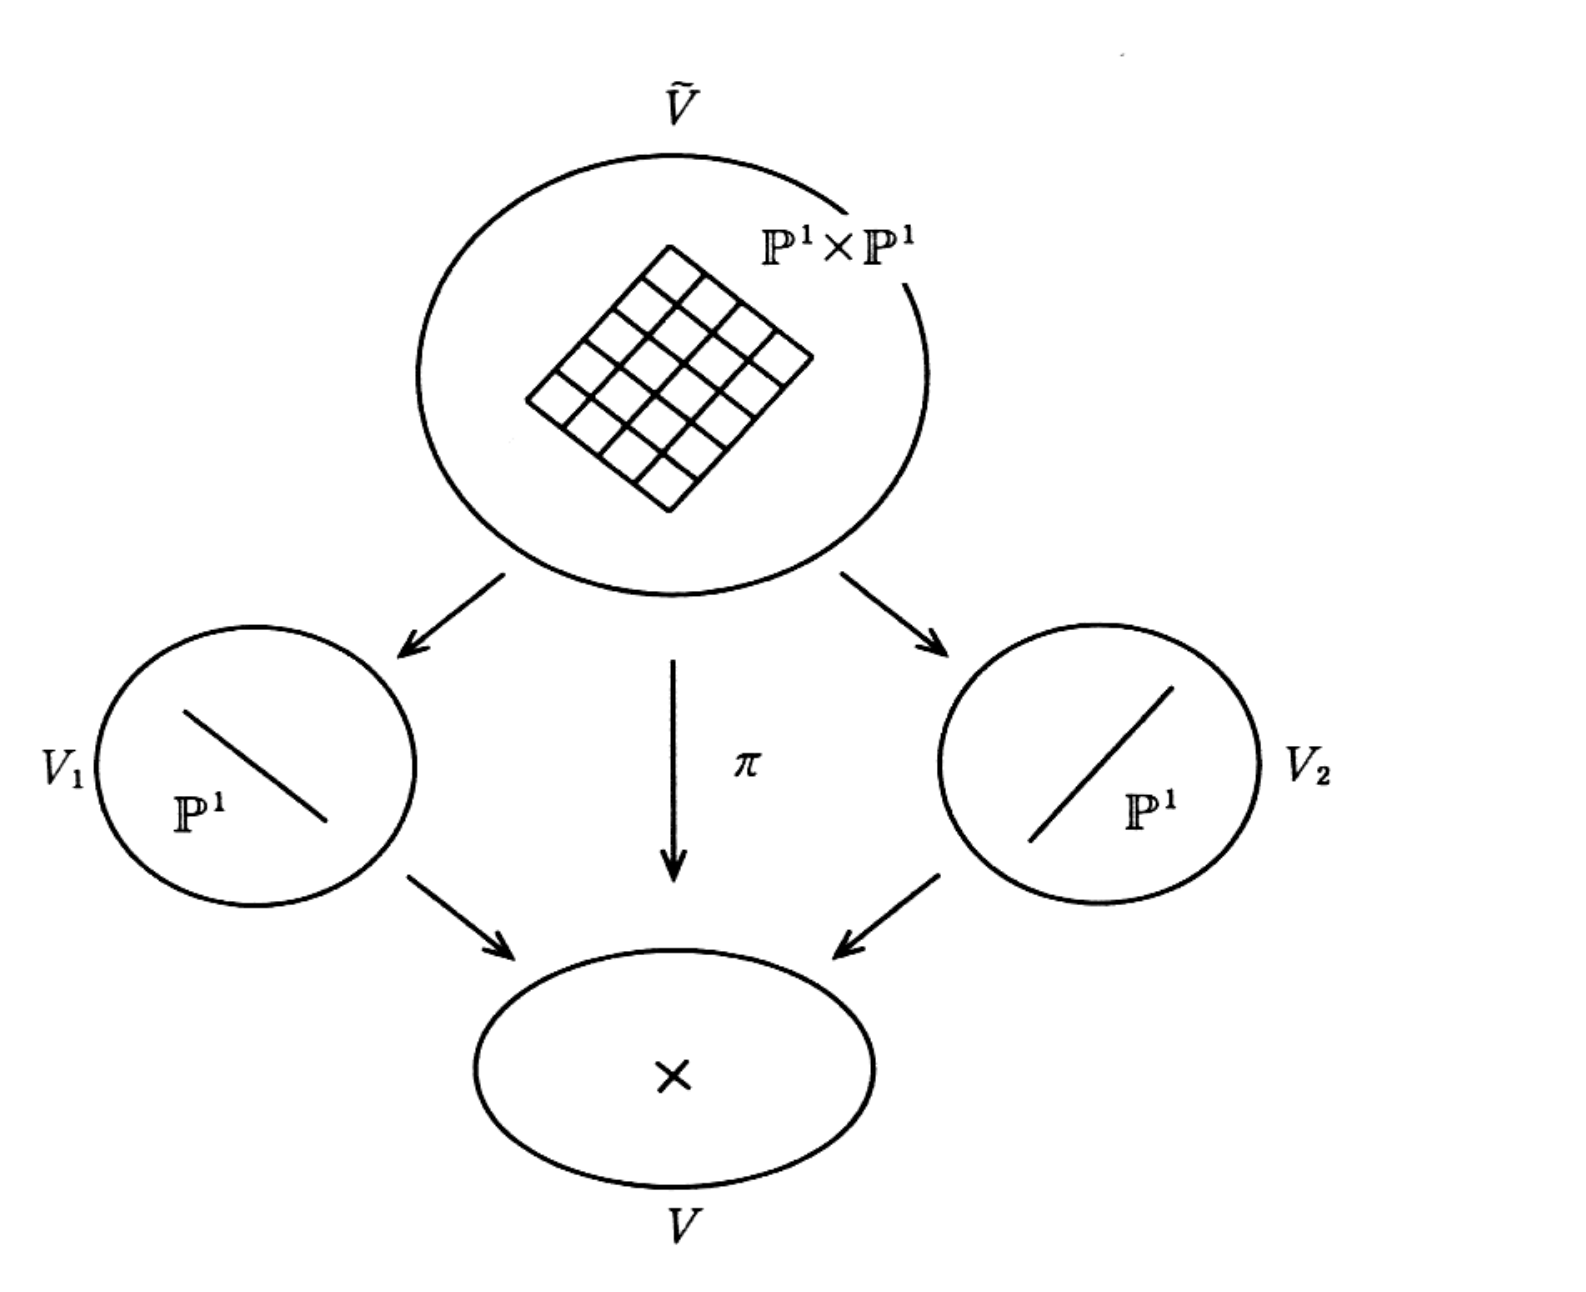
\includegraphics[width=0.72\linewidth]{figures/ch04-fig1.png}
  \figtitle{1}{$V$ 的小消解 $V_1,V_2$ 与 $\tilde{V}\to V$（原书 p.57）}
\end{figure}

\begin{figure}[htbp]
  \centering
  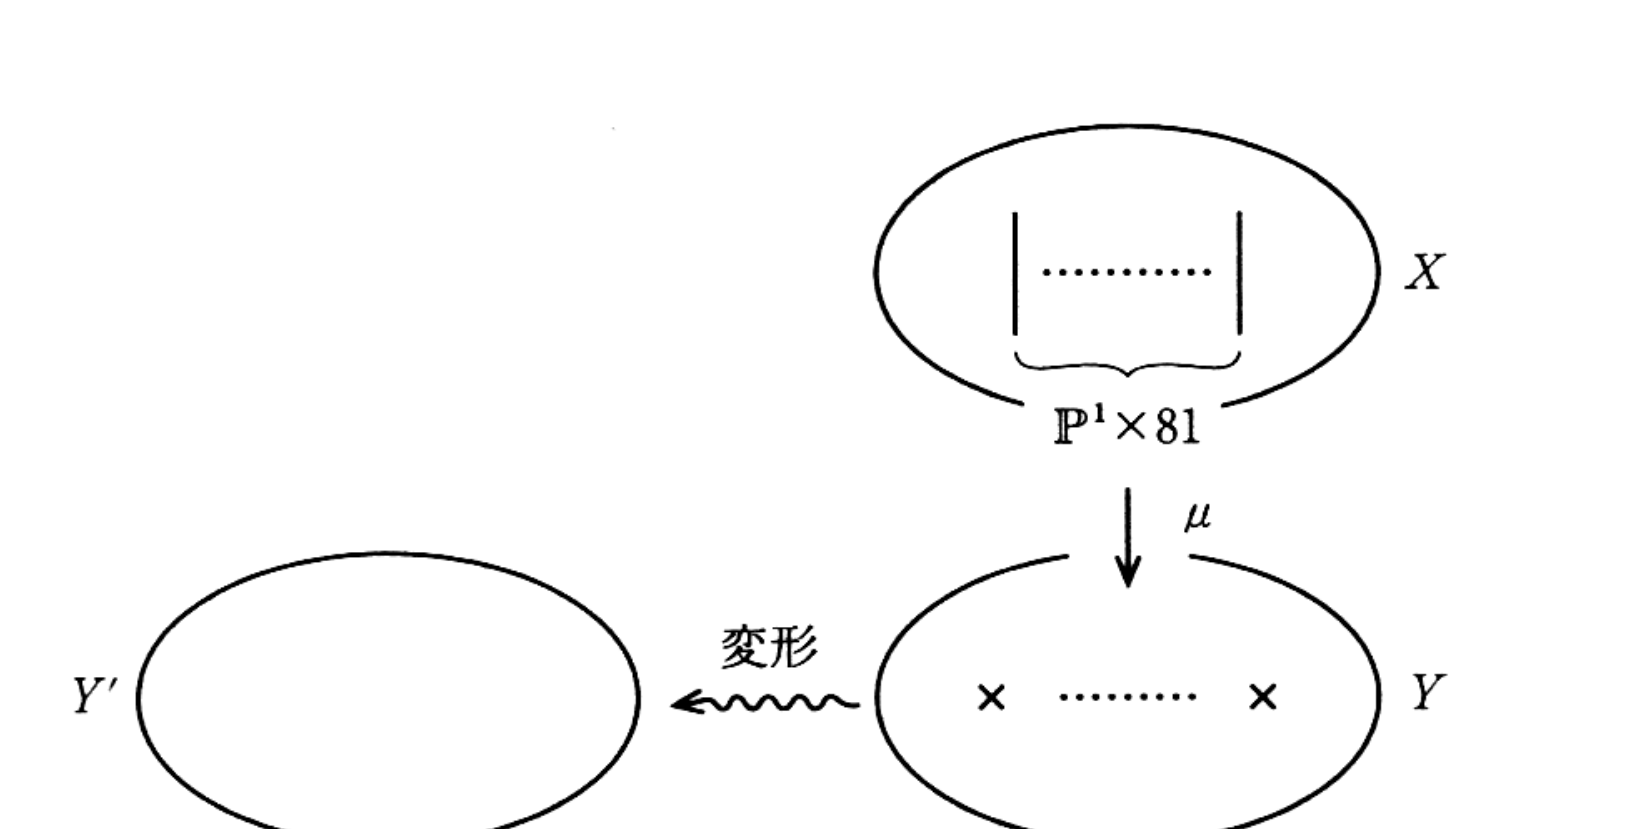
\includegraphics[width=0.86\linewidth]{figures/ch04-fig2.png}
  \figtitle{2}{锥形流形跃迁：$X$ 经 $\mu$ 收缩到 $Y$，再形变到 $Y'$（原书 p.57）}
\end{figure}

% [Tutor Note: 原书此页两幅图没有图题，图 1、图 2 的编号与题注为译者所加。图 1 中 $\tilde{V}$ 内的网格示意例外除子 $\PP^1\times\PP^1$；图 2 中的「変形」即“形变”，箭头表示锥形流形跃迁的第二步。]

不用锥形流形，而用具有典范奇点的 Calabi--Yau 流形，也可以考虑同样的操作（这里姑且叫作带奇点的 Calabi--Yau 跃迁）。不过这时，会直面带奇点的 Calabi--Yau 流形何时能通过形变变成非奇异的问题。关于这一点，作者与 Gross 已经得到若干结果，但这里省略。

Reid 的幻想（Reid's fantasy），说的是下面的猜想（与其说是猜想，不如说是梦想）。

% ===== PDF p.066 (原书 p.58) =====
% [Tutor Note: 这就是所谓的 Reid 的幻想：把 3 维 Calabi--Yau 流形的“形变”与“带奇点的 Calabi--Yau 跃迁”两种操作反复施行，就能把任意两个 3 维单连通 Calabi--Yau 流形连起来。若为真，则 3 维单连通 Calabi--Yau 流形的双有理等价类可以连成一张“网”。]

\begin{conjecture}{}
  两个 3 维单连通 Calabi--Yau 流形，通过反复施行形变与带奇点的 Calabi--Yau 跃迁这两种操作，可以相连。
\end{conjecture}

\section{其他未解决的问题}

最后介绍两个未解决的问题，以结束本次的讨论。

\begin{problem}{}
  单连通的 Calabi--Yau 流形含有理曲线吗？
\end{problem}

这个问题与 Calabi--Yau 流形的 Gromov--Witten 不变量有很深的关系。这里所说的有理曲线，是指正规化（奇点消解）后成为 $\PP^1$ 的代数曲线。对代数的 $K3$ 曲面，这个问题的答案是肯定的。因此问题出在 3 维以上的情形。对 Fano 流形，森理论是有效的，但典范丛平凡时，就不知道怎样才能找出有理曲线。另外，加进单连通这个假设，是为了排除那些取平展覆盖后就成为阿贝尔簇的 Calabi--Yau 流形。

\begin{problem}{}
  对 3 维 Calabi--Yau 流形 $X$，与 $X$ 双有理等价的 Calabi--Yau 流形的同构类的个数有限吗？
\end{problem}

这个问题与极小模型问题有很深的关系。在 3 维，一个双有理类中存在多个极小模型。不同的极小模型由叫作 flop 的变换联系起来。因此这里成问题的那些 Calabi--Yau 流形，就是对 $X$ 施行若干次 flop 得到的流形。另外，Morrison 提出了关于 Calabi--Yau 流形的 Kähler 锥的猜想（锥猜想）。这些猜想似乎也与镜像猜想有关。

% ===== PDF p.067 (原书 p.59) =====
\begin{reflist}
  \item[{}] 关于代数簇的分类理论，可举出下面这些启蒙性的文献。
  \item[{[1]}] 『数学セミナー』1997 年 12 月号特集「小平邦彦」
  \item[{}] 想更正规地学习的人，可参看下面的文献。
  \item[{[2]}] Ueno, K.: \textit{Classification theory of algebraic varieties and compact complex spaces}, Lecture Notes in Math. 439, Springer-Verlag.
  \item[{[3]}] Wilson, P. M. H.: \textit{Towards birational classification of algebraic varieties}, Bull. London Math. Soc. \textbf{19} (1987), 1--48.
  \item[{}] 读一读 [2]、[3]，大概就能很好地理解 Calabi--Yau 流形在代数簇中处于什么位置。Calabi--Yau 流形的形变理论、用环簇几何构造镜像流形等内容，在下面的文献中有简洁的介绍。
  \item[{[4]}] Voisin, C.: \textit{Symétris miroir}, Panoramas et Synthèses 2, Soc. Math. de France, Paris, 1996.
  \item[{}] [4] 似乎还有美国数学会出版的英译本。
\end{reflist}

% 本章节号至此结束，恢复 preamble 的罗马数字默认，避免影响 ch05 及以后。
\renewcommand{\thesection}{\Roman{section}}

